\pdfminorversion=4
\documentclass[aspectratio=169]{beamer}

\mode<presentation>
{
  \usetheme{default}
  \usecolortheme{default}
  \usefonttheme{default}
  \setbeamertemplate{navigation symbols}{}
  \setbeamertemplate{caption}[numbered]
  \setbeamertemplate{footline}[frame number]  % or "page number"
  \setbeamercolor{frametitle}{fg=white}
  \setbeamercolor{footline}{fg=black}
} 

\usepackage[english]{babel}
\usepackage{inputenc}
\usepackage{tikz}
\usepackage{courier}
\usepackage{array}
\usepackage{bold-extra}
\usepackage{minted}
\usepackage[thicklines]{cancel}
\usepackage{fancyvrb}

\xdefinecolor{ucred}{rgb}{0.50,0,0}
\xdefinecolor{dianablue}{rgb}{0.18,0.24,0.31}
\xdefinecolor{darkblue}{rgb}{0.1,0.1,0.7}
\xdefinecolor{darkgreen}{rgb}{0,0.5,0}
\xdefinecolor{darkgrey}{rgb}{0.35,0.35,0.35}
\xdefinecolor{darkorange}{rgb}{0.8,0.5,0}
\xdefinecolor{darkred}{rgb}{0.7,0,0}
\definecolor{darkgreen}{rgb}{0,0.6,0}
\definecolor{mauve}{rgb}{0.58,0,0.82}

\title[2025-07-12-scipy-teen-track]{\textcolor{black}{SciPy 2025 Teen Track project: data science and voting rights}}
\author{Jim Pivarski}
\institute{University of Chicago -- Data Science Institute}
\date{July 12, 2025}

\usetikzlibrary{shapes.callouts}

\begin{document}

\logo{\pgfputat{\pgfxy(0.11, 7.4)}{\pgfbox[right,base]{\tikz{\filldraw[fill=ucred, draw=none] (0 cm, 0 cm) rectangle (50 cm, 1 cm);}\mbox{\hspace{-8 cm}
\includegraphics[height=1 cm]{uchicago-logo-long.png}\hspace{0.1 cm}{
\includegraphics[height=1 cm]{dsi-logo-long.png}}\hspace{0.1 cm}}}}}

\begin{frame}
  \titlepage
\end{frame}

\logo{\pgfputat{\pgfxy(0.11, 7.4)}{\pgfbox[right,base]{\tikz{\filldraw[fill=ucred, draw=none] (0 cm, 0 cm) rectangle (50 cm, 1 cm);}\mbox{\hspace{-8 cm}
\includegraphics[height=1 cm]{uchicago-logo.png}{
\includegraphics[height=1 cm]{dsi-logo.png}}\hspace{0.1 cm}}}}}

% Uncomment these lines for an automatically generated outline.
%\begin{frame}{Outline}
%  \tableofcontents
%\end{frame}

% START START START START START START START START START START START START START

\begin{frame}{Who am I?}
\vspace{0.5 cm}
\begin{itemize}
\item<1-> Particle physicist: helped get the LHC ready to discover the Higgs boson, did some precision studies and some exotic particle searches (didn't find any!).
\item<2-> Data scientist: mid-career detour, or rather a back-and-forth between commercial, academic, and now philanthropic data science.
\end{itemize}

\vspace{0.25 cm}
\uncover<3->{\textcolor{darkblue}{$\longrightarrow$ A science/math/computing education doesn't lock you into a specific career.}}

\vspace{0.25 cm}
\begin{columns}
\column{1.1\linewidth}
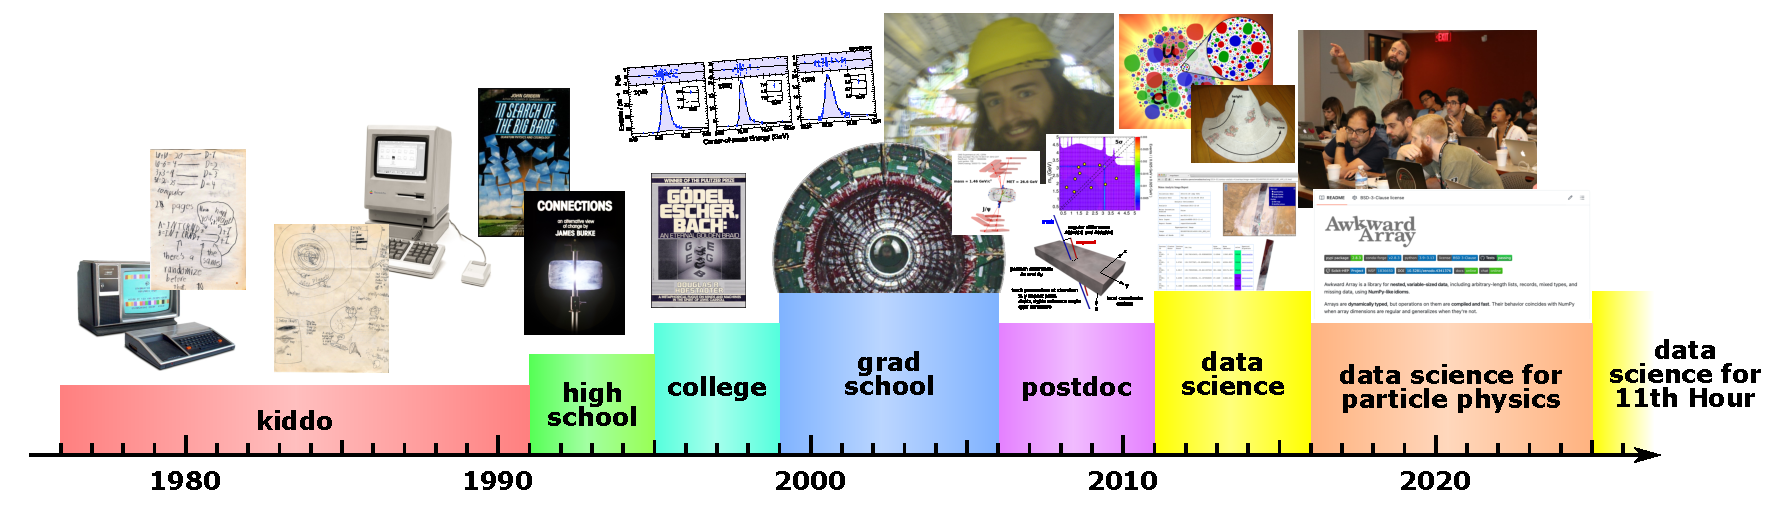
\includegraphics[width=\linewidth]{img/personal-timeline.pdf}
\end{columns}
\end{frame}

\begin{frame}{The 11th Hour Project}
\vspace{0.25 cm}
\begin{columns}
\column{0.36\linewidth}
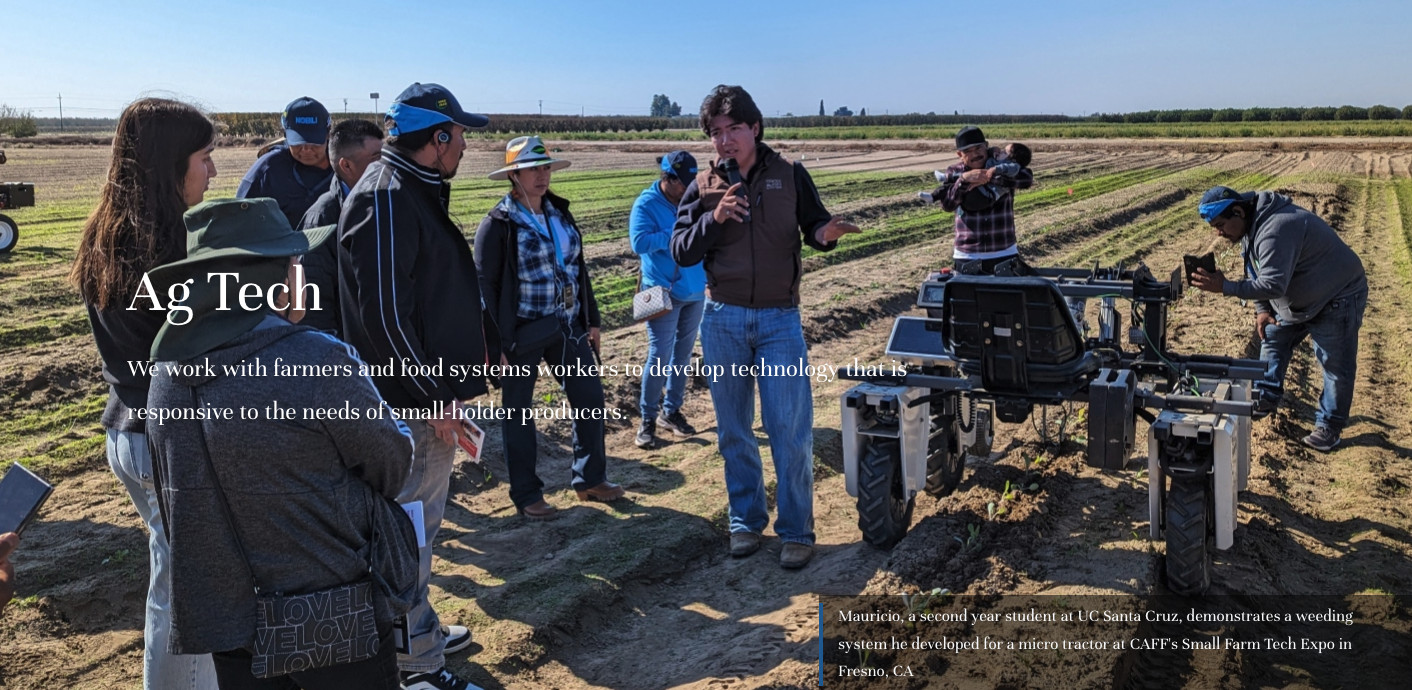
\includegraphics[width=\linewidth]{img/11thhour-1.jpg}

\vspace{0.15 cm}
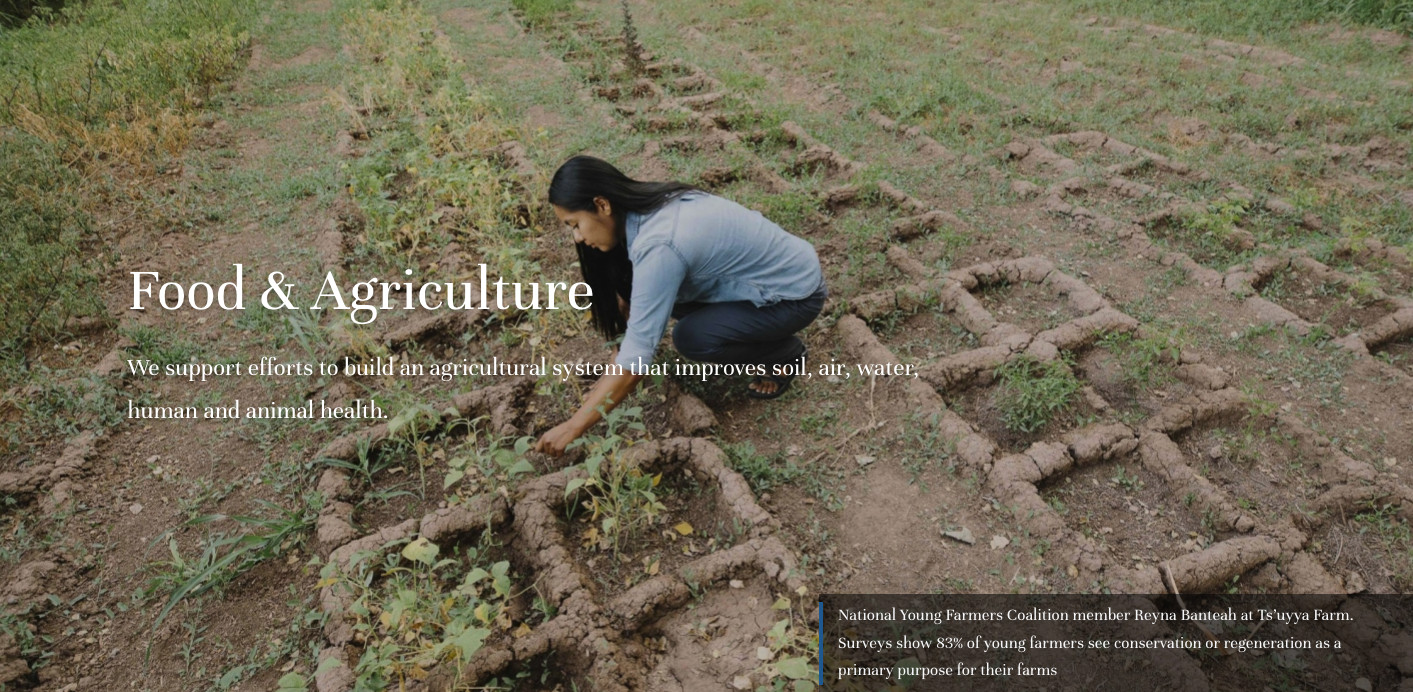
\includegraphics[width=\linewidth]{img/11thhour-4.jpg}

\vspace{0.15 cm}
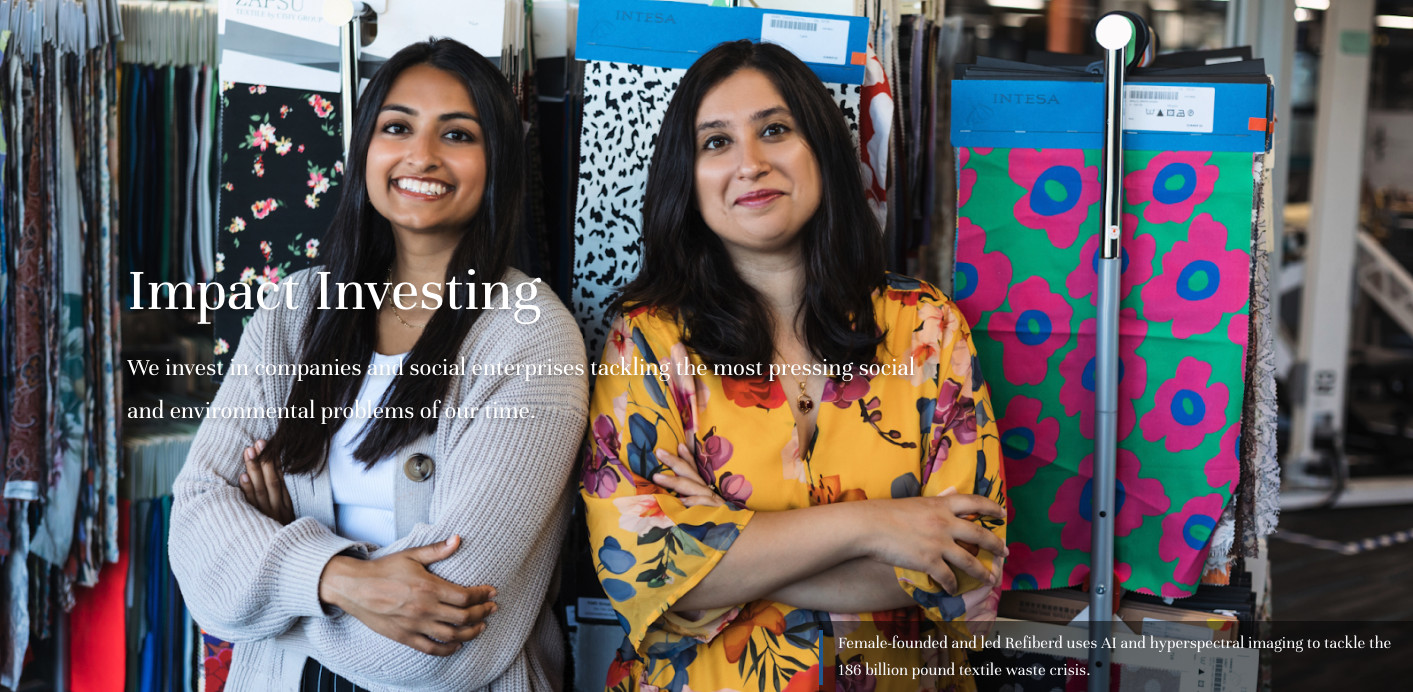
\includegraphics[width=\linewidth]{img/11thhour-7.jpg}

\column{0.36\linewidth}
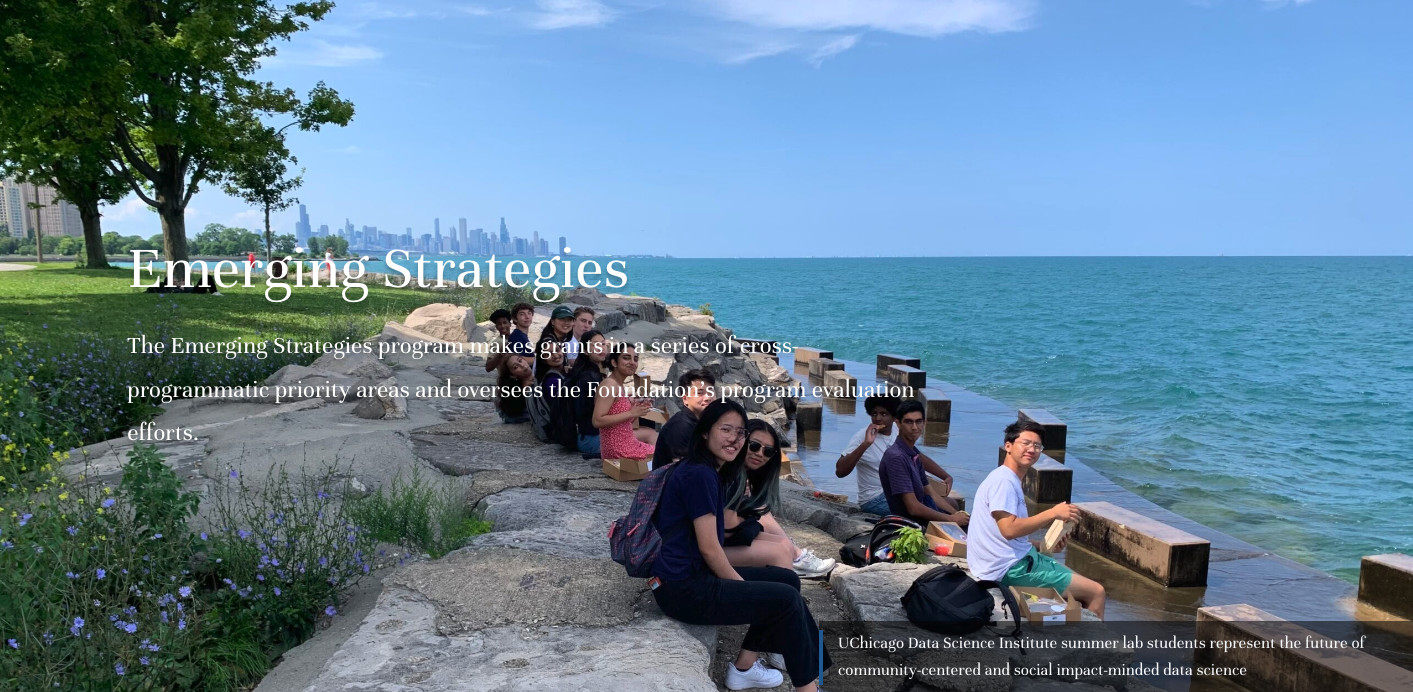
\includegraphics[width=\linewidth]{img/11thhour-2.jpg}

\vspace{0.15 cm}
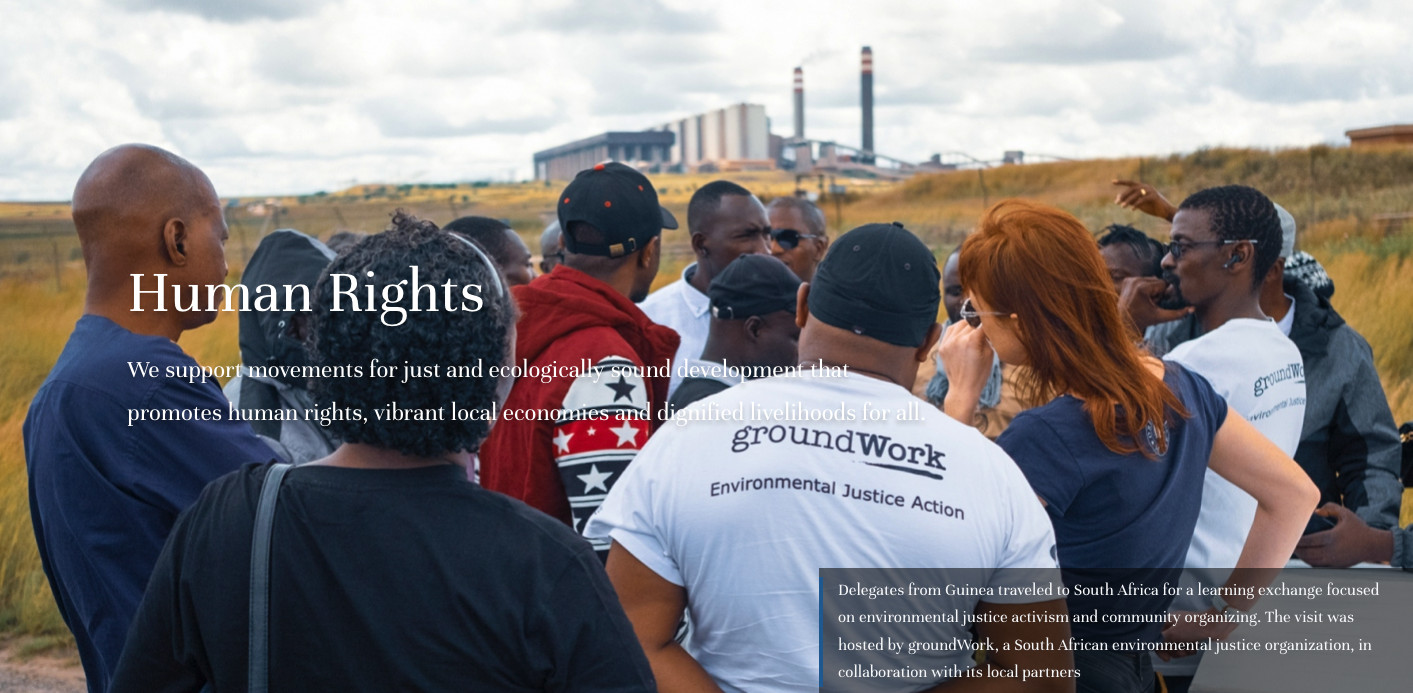
\includegraphics[width=\linewidth]{img/11thhour-5.jpg}

\vspace{0.15 cm}
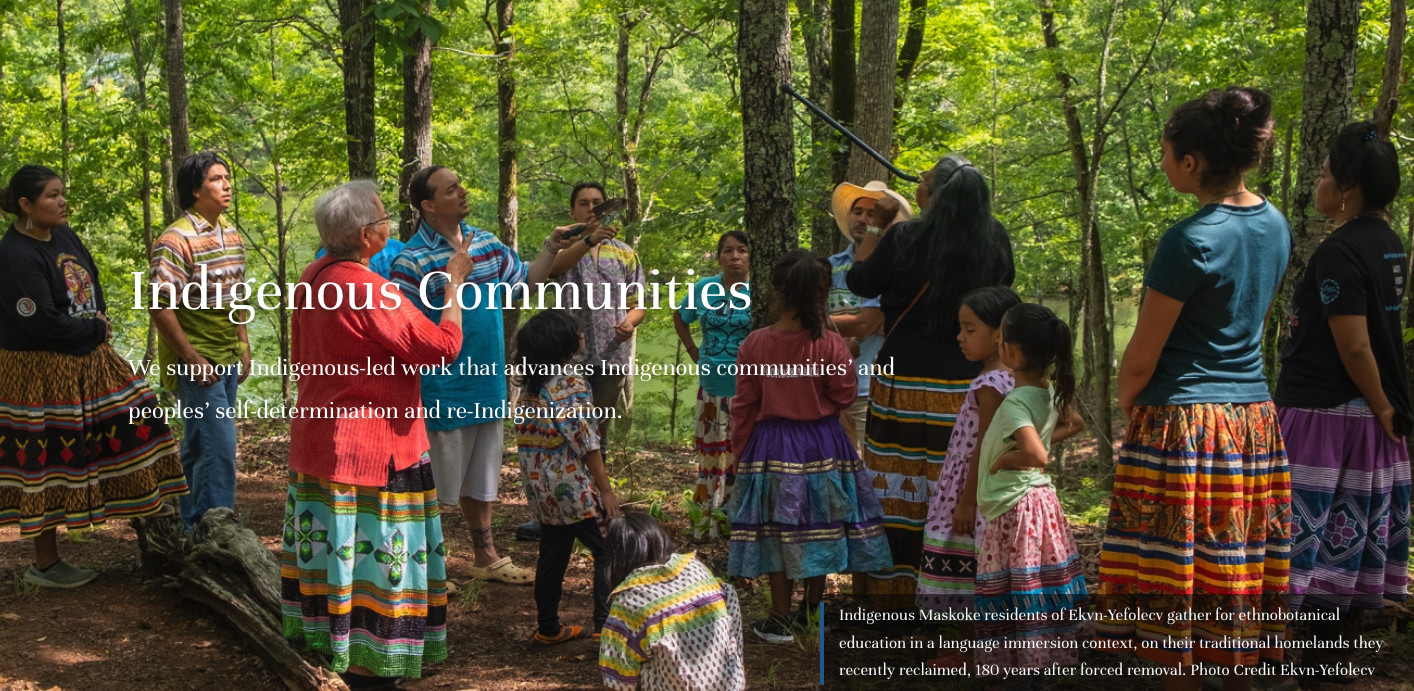
\includegraphics[width=\linewidth]{img/11thhour-8.jpg}

\column{0.36\linewidth}
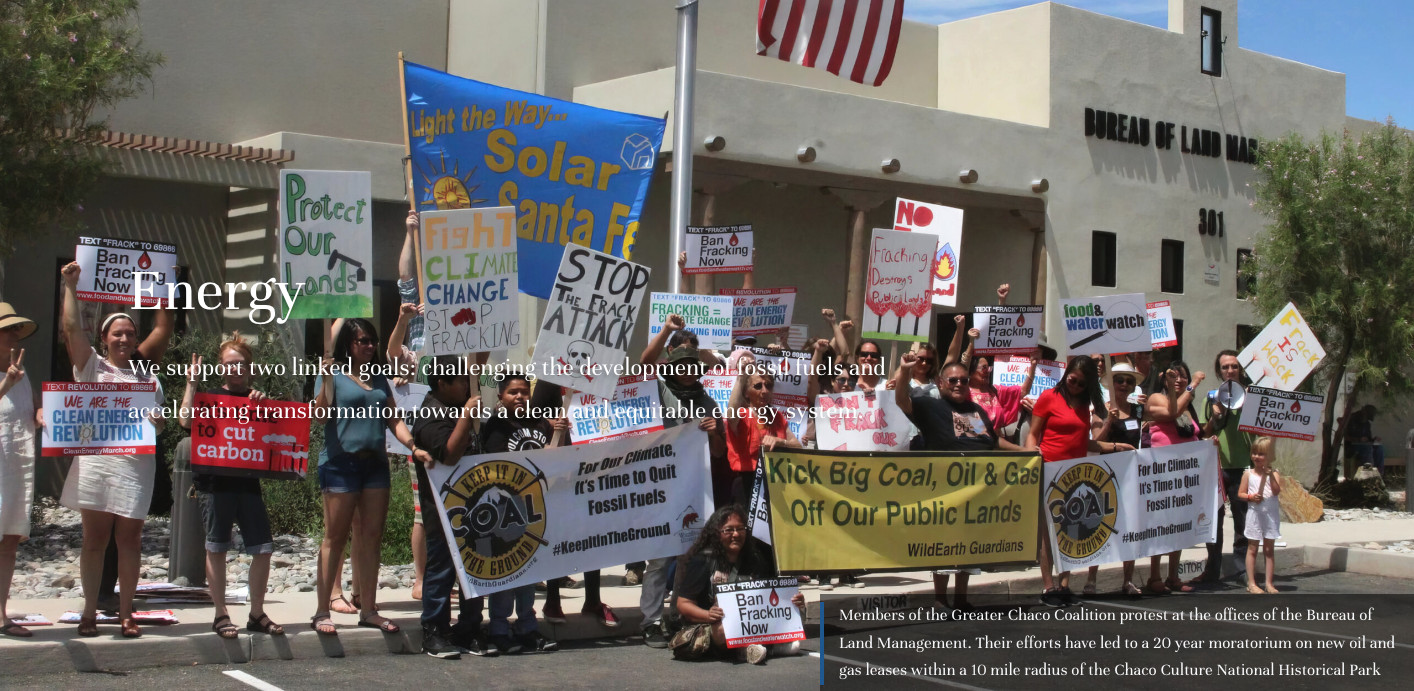
\includegraphics[width=\linewidth]{img/11thhour-3.jpg}

\vspace{0.15 cm}
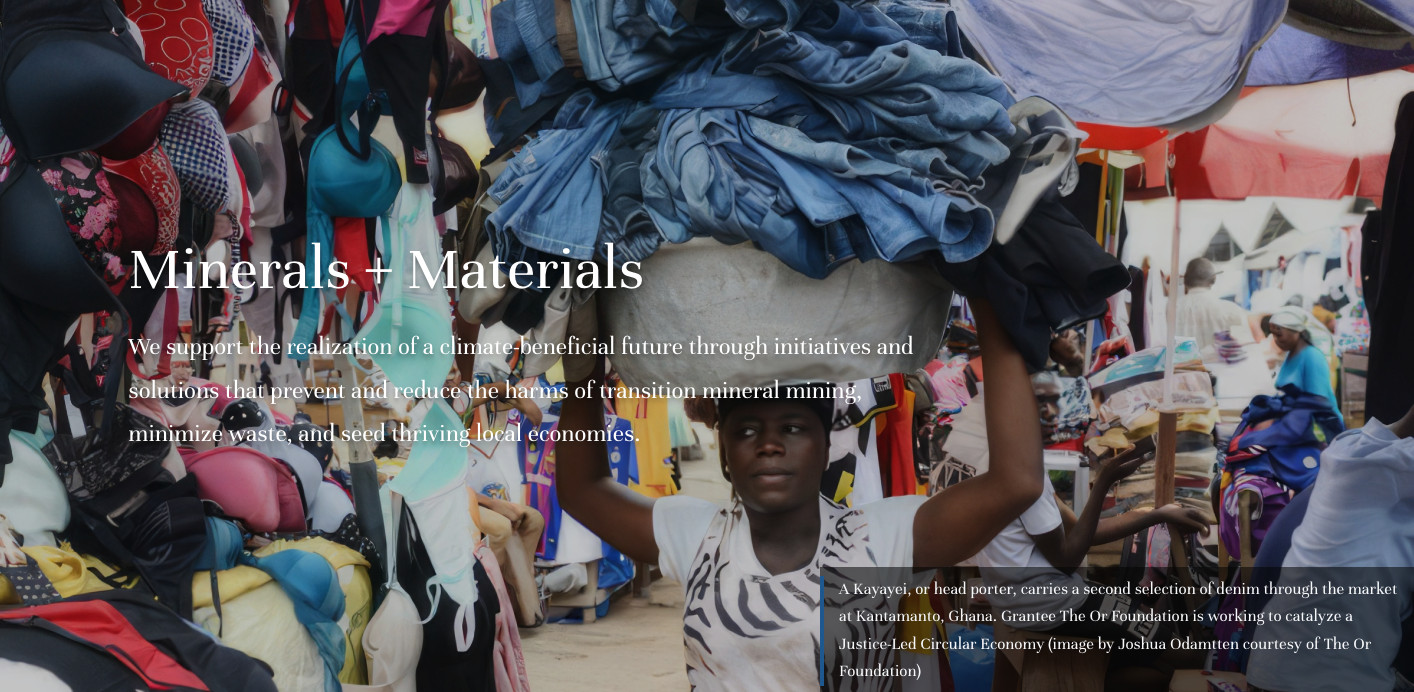
\includegraphics[width=\linewidth]{img/11thhour-6.jpg}

\vspace{0.15 cm}
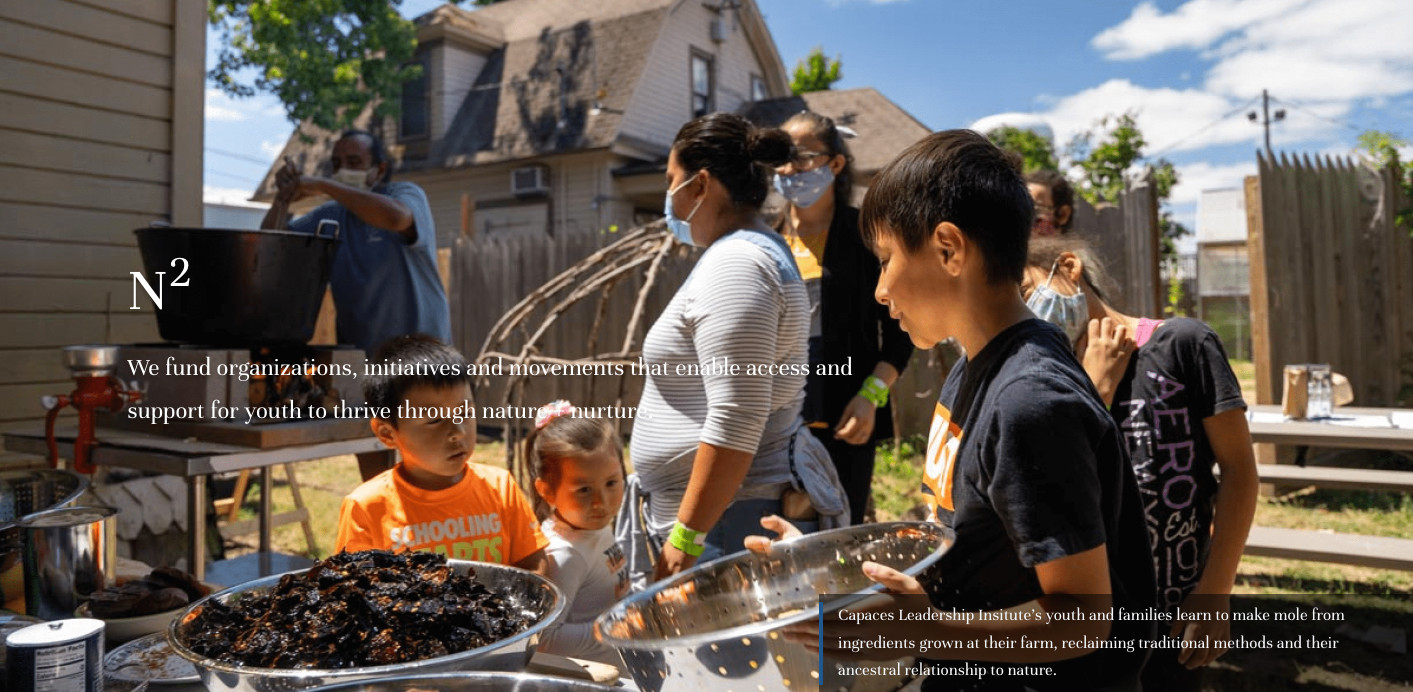
\includegraphics[width=\linewidth]{img/11thhour-9.jpg}
\end{columns}
\end{frame}

\begin{frame}{Universtiy of Chicago's Data Science Institute (DSI)}
\vspace{0.35 cm}
\begin{columns}
\column{0.85\linewidth}
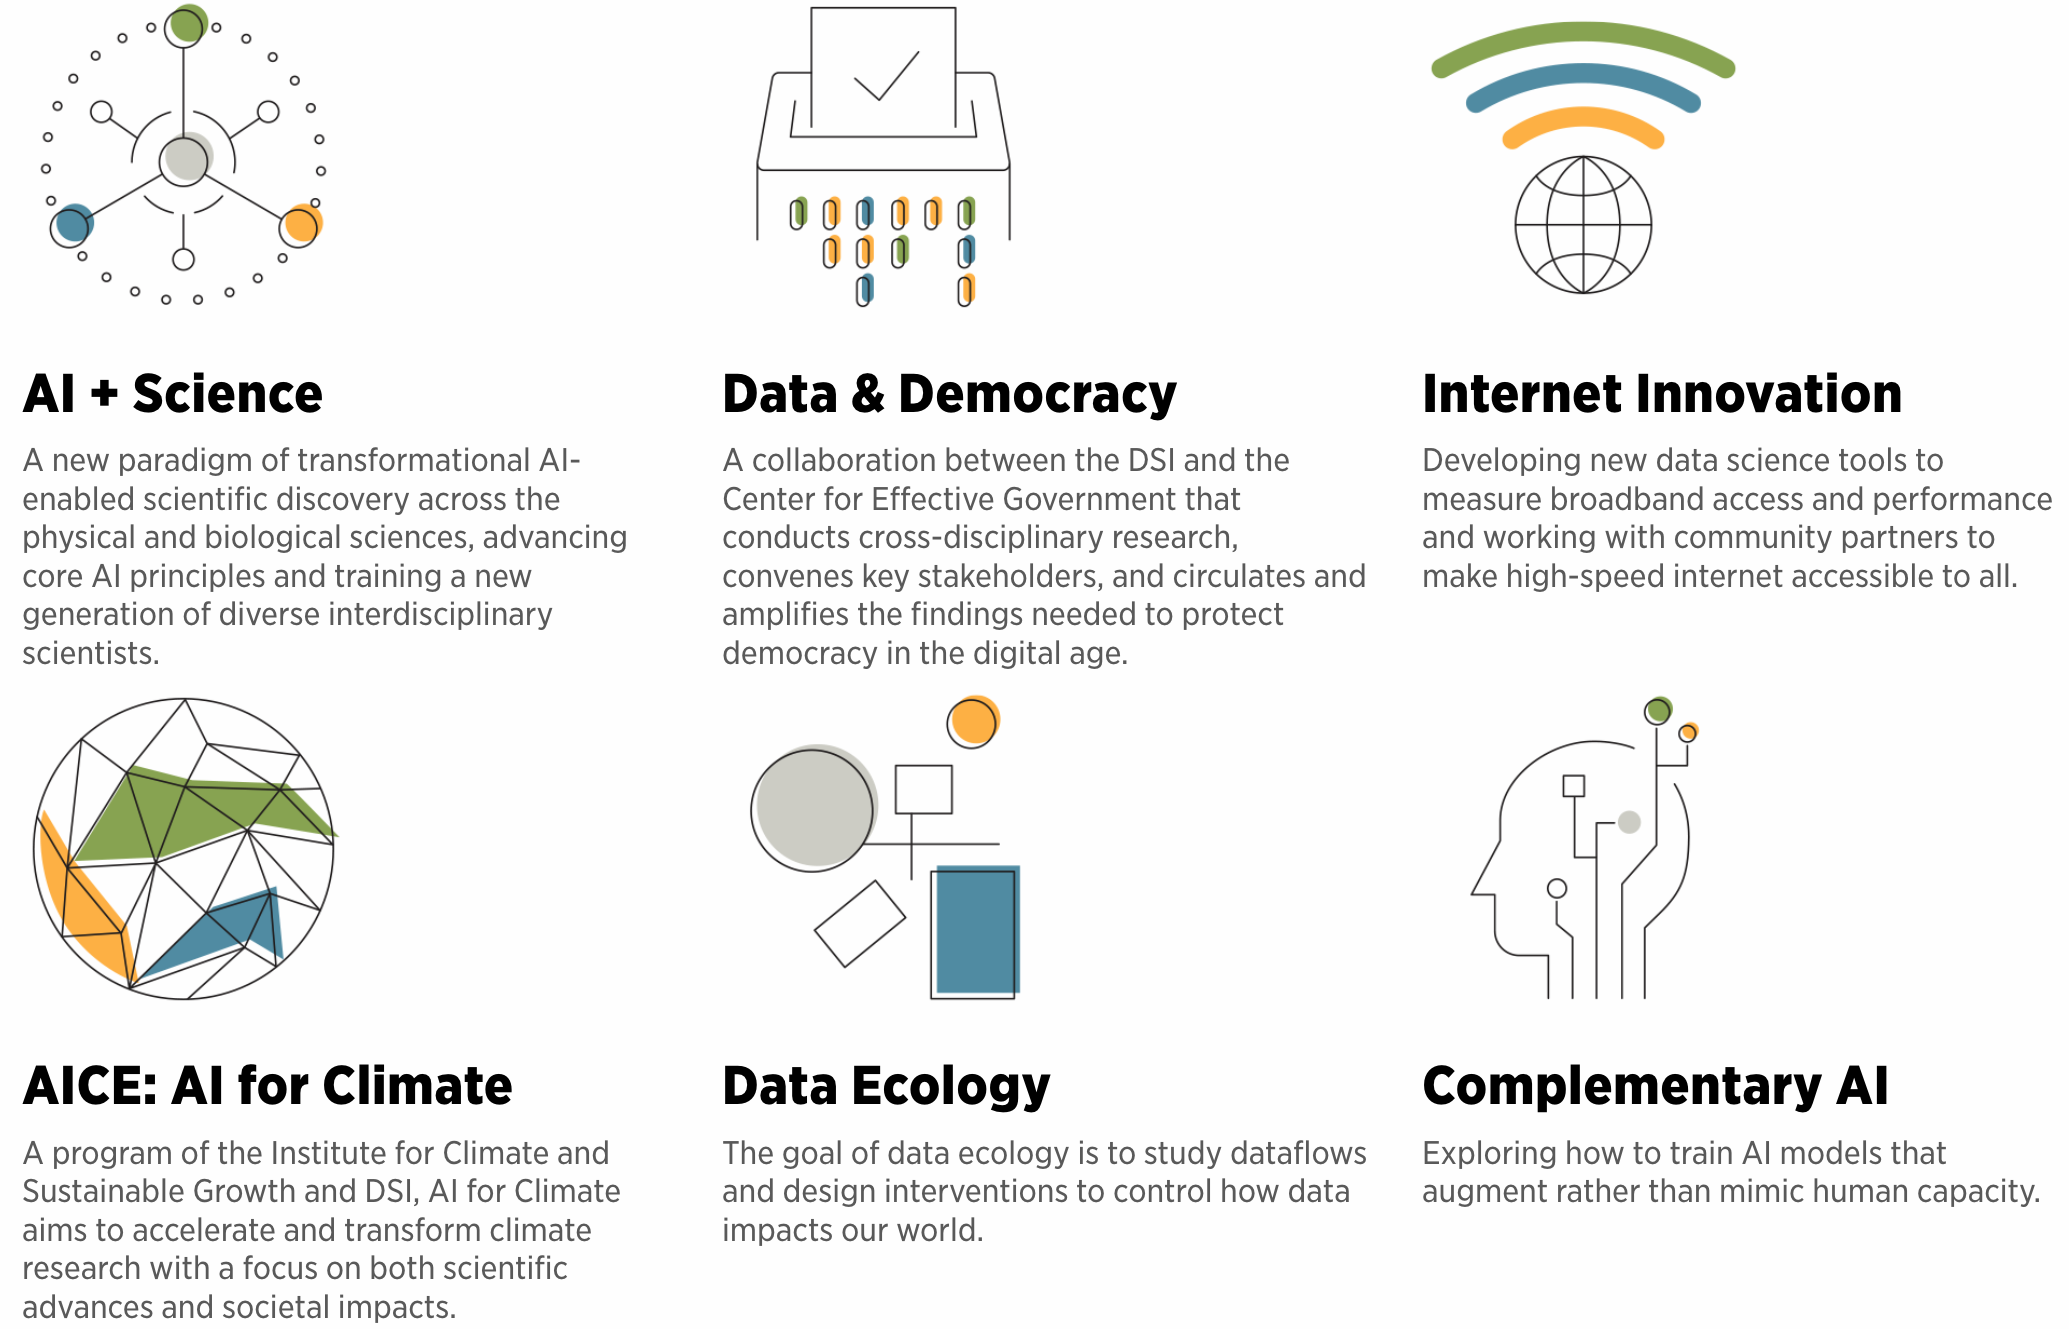
\includegraphics[width=\linewidth]{img/uchicago-dsi-website.png}
\end{columns}
\end{frame}

\begin{frame}{I'm part of a group within the DSI that helps 11th Hour projects}
\vspace{0.25 cm}
\begin{columns}
\column{0.87\linewidth}
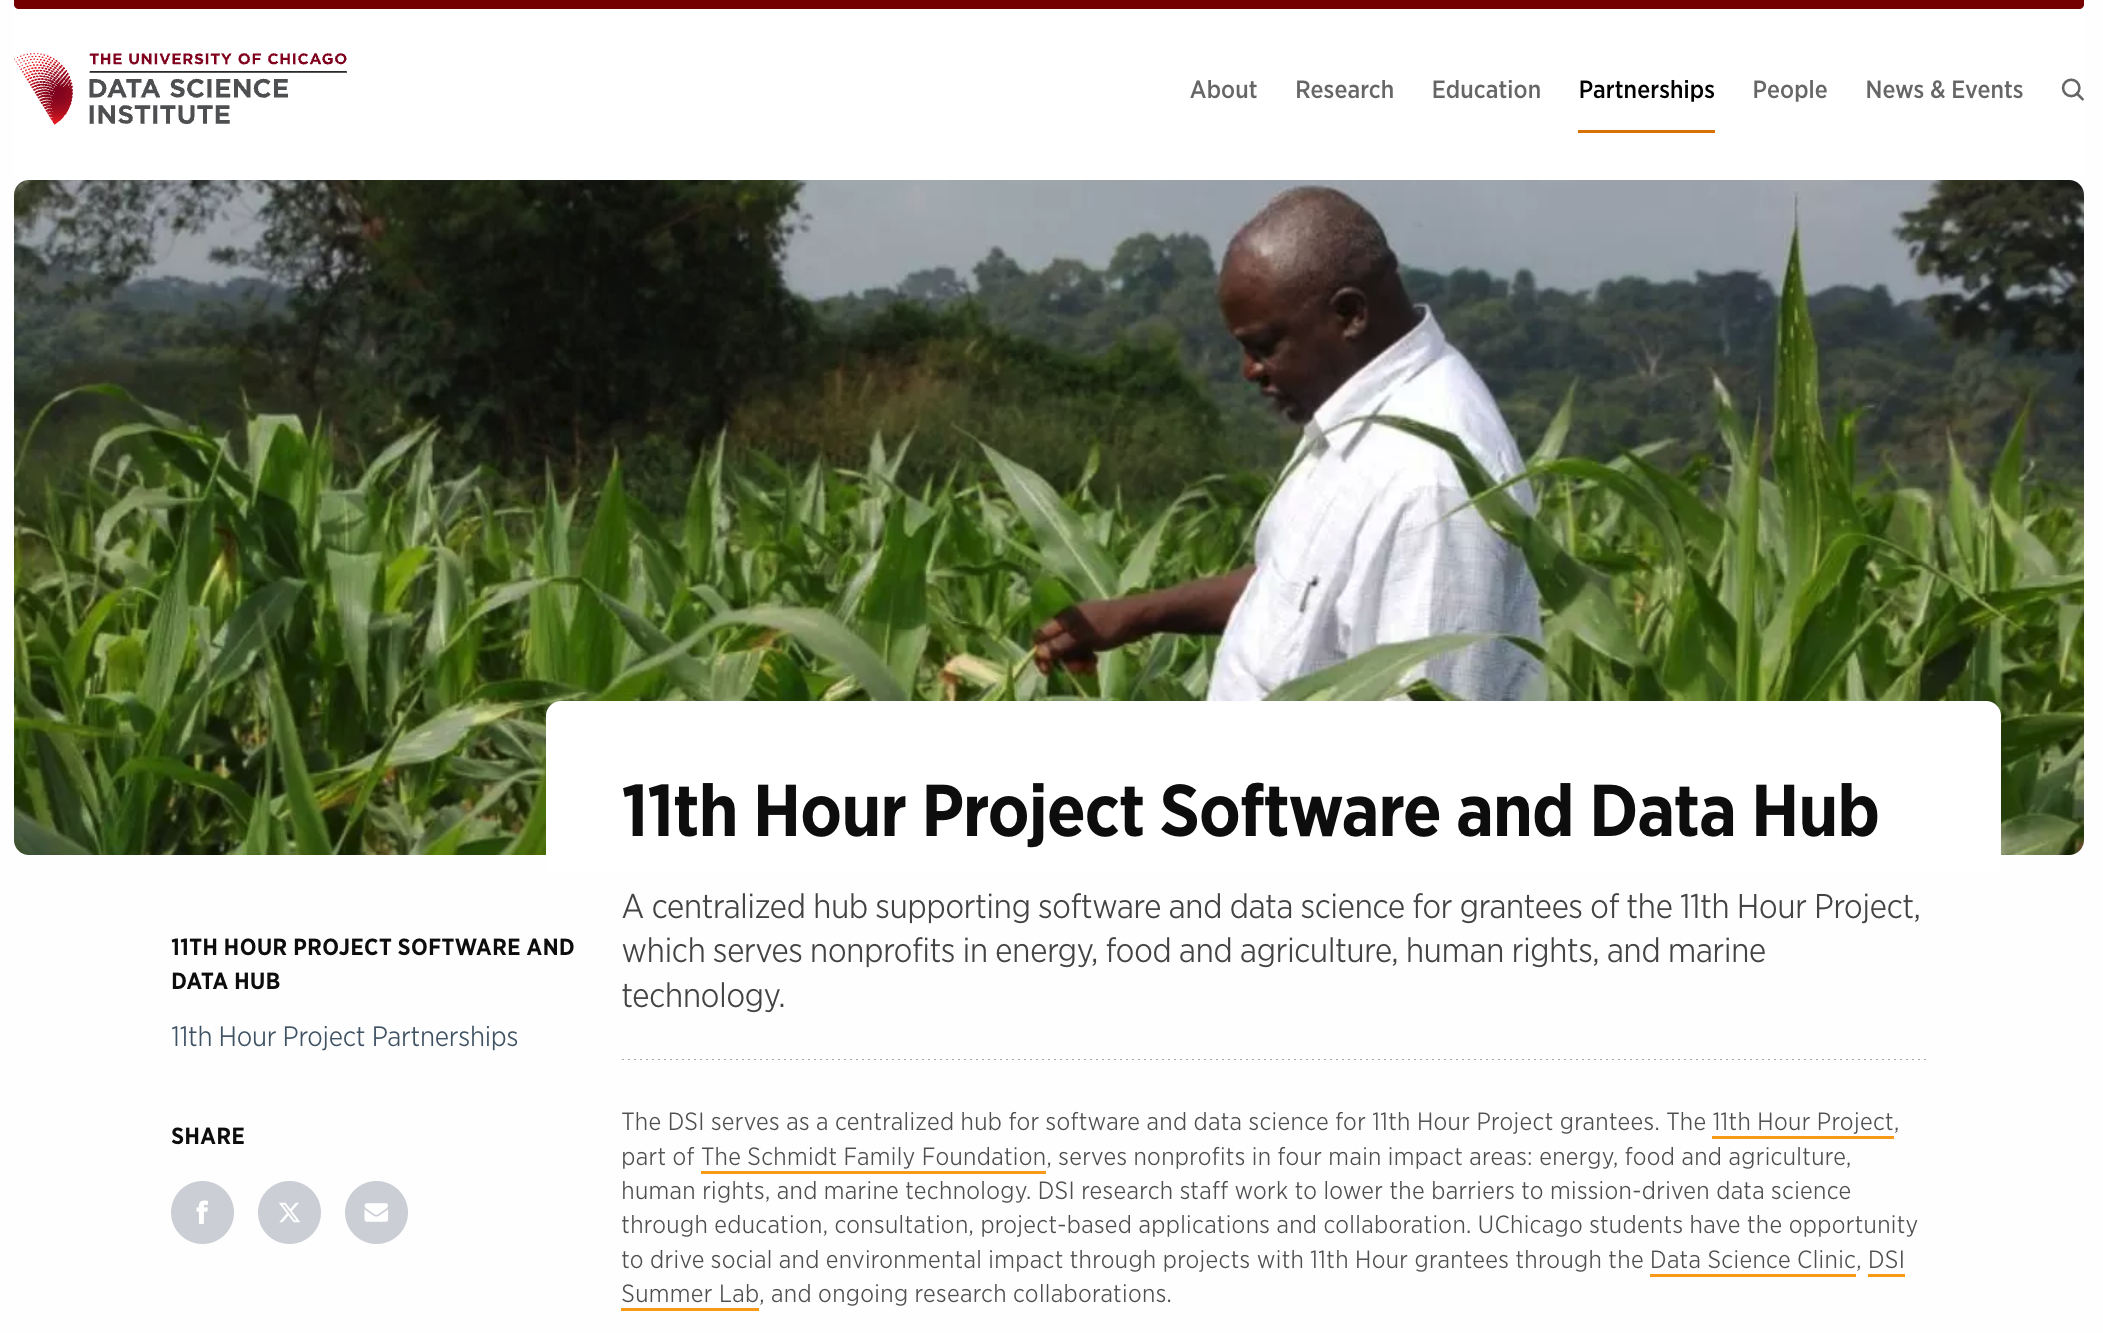
\includegraphics[width=\linewidth]{img/uchicago-dsi-11thhour-website.png}
\end{columns}
\end{frame}

\begin{frame}{Recent project: North Dakota Native Vote}
\vspace{0.35 cm}
\begin{columns}
\column{0.97\linewidth}
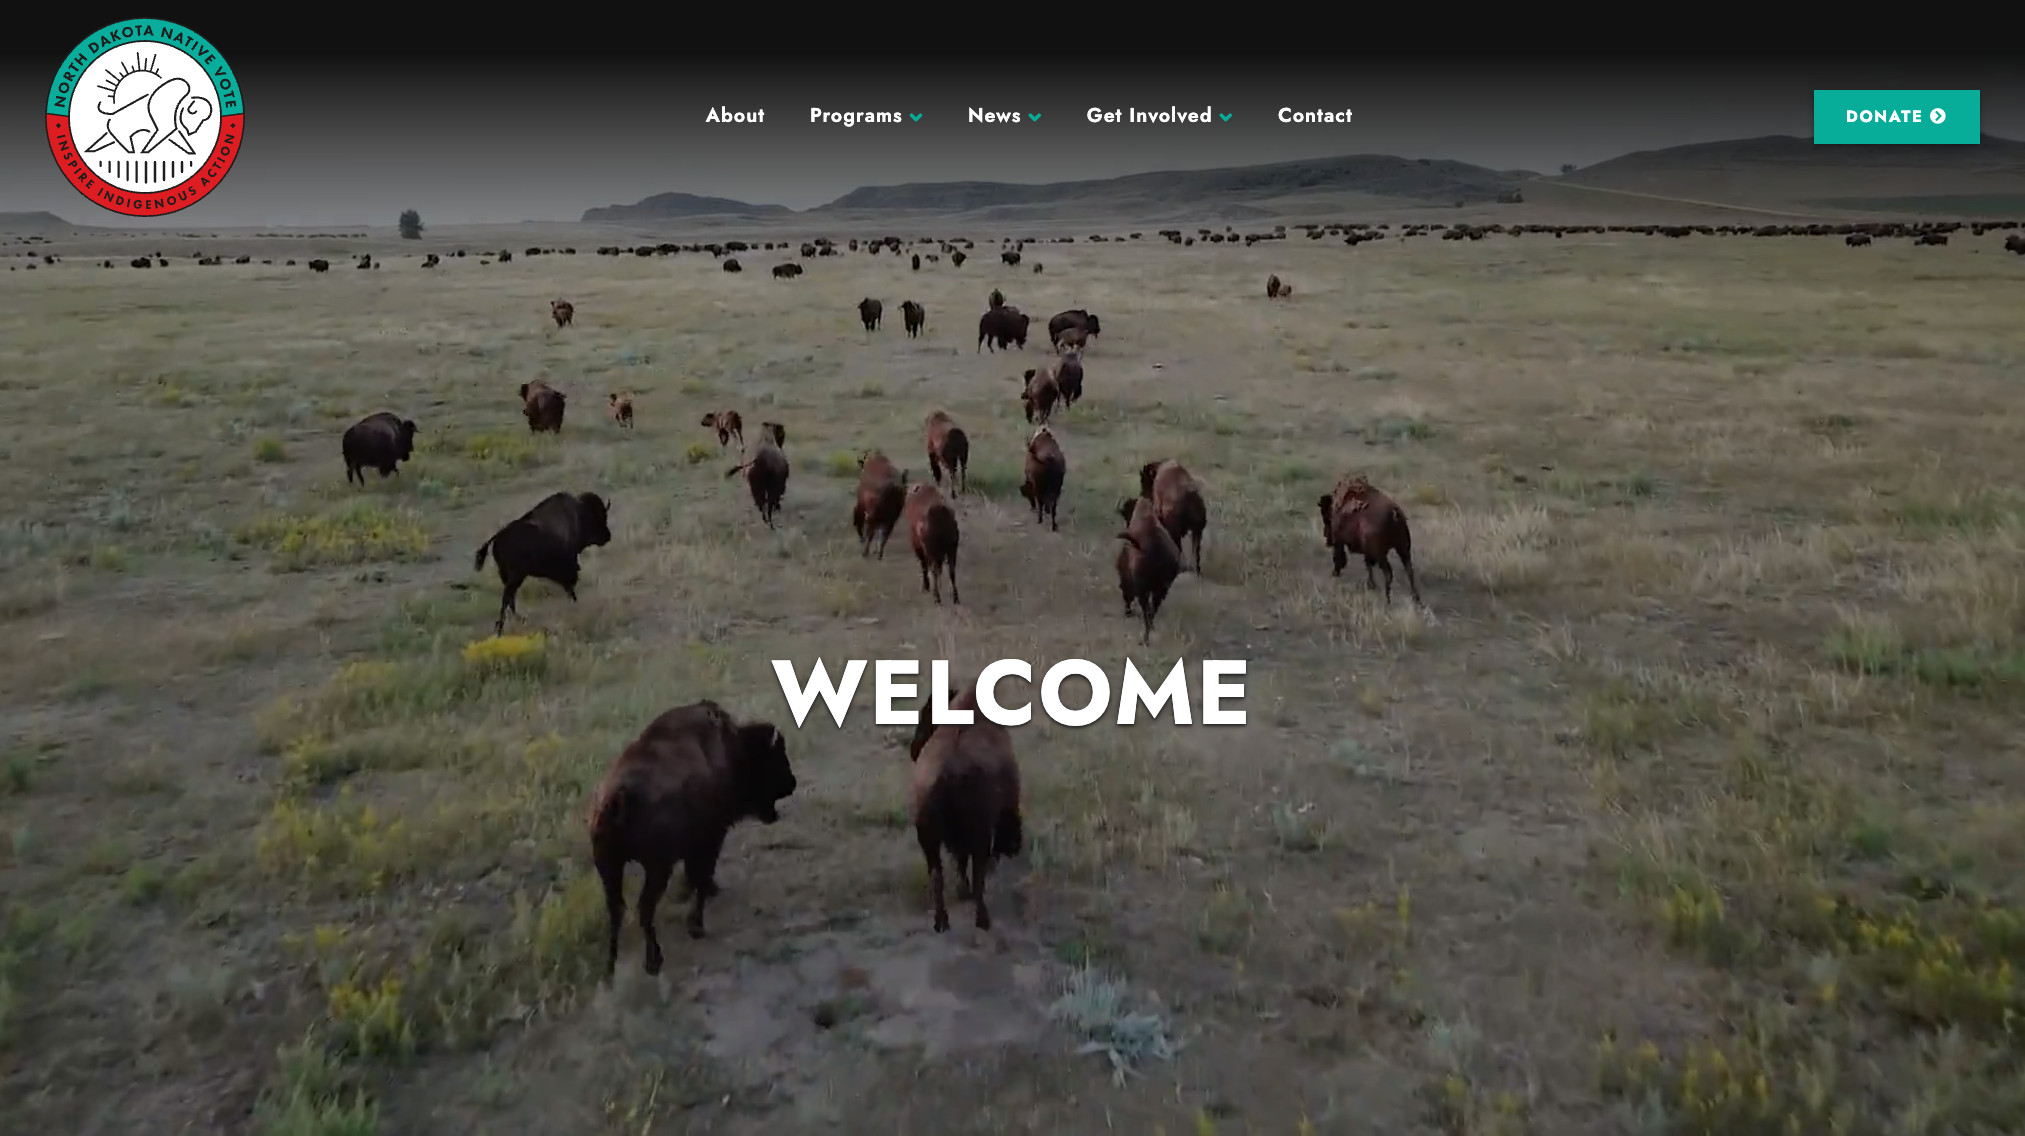
\includegraphics[width=\linewidth]{img/ndnativevote-website.jpg}
\end{columns}
\end{frame}

\begin{frame}{Problems that keep Native Americans from voting}
\vspace{0.5 cm}
\begin{itemize}\setlength{\itemsep}{0.5 cm}
\item<1-> New voter ID requirement in North Dakota.
\begin{itemize}
\item<2-> People without a house number on their tribal ID card are turned away at the polls.
\item<3-> The U.S. mail doesn't deliver to most houses on reservations, so house numbers aren't in common use---most people don't know their full address.
\item<4-> Addresses do exist (maintained by the 911 commissioners), so this is a data access problem that we're working on.
\end{itemize}
\item<5-> Long distance to polls (up to 80 miles!), gas money, time off work, daycare.
\item<6-> Distrust, due to historical disenfranchisement. \\ (It wasn't until 1958 that voting became legal for tribes in North Dakota!)
\item<7-> Gerrymandering. Recently, the Turtle Mountain Chippewa and Spirit Lake Sioux scored a major victory in overturning a blatant case of gerrymandering:
\begin{itemize}\scriptsize
\item \textcolor{blue}{\url{https://narf.org/cases/north-dakota-redistricting-map/}}
\item \textcolor{blue}{\url{https://ndnativevote.org/wp-content/uploads/Redistricting-Guide.pdf}}
\end{itemize}
\end{itemize}
\end{frame}

\begin{frame}{What is gerrymandering?}
\vspace{0.25 cm}
\begin{columns}
\column{0.55\linewidth}
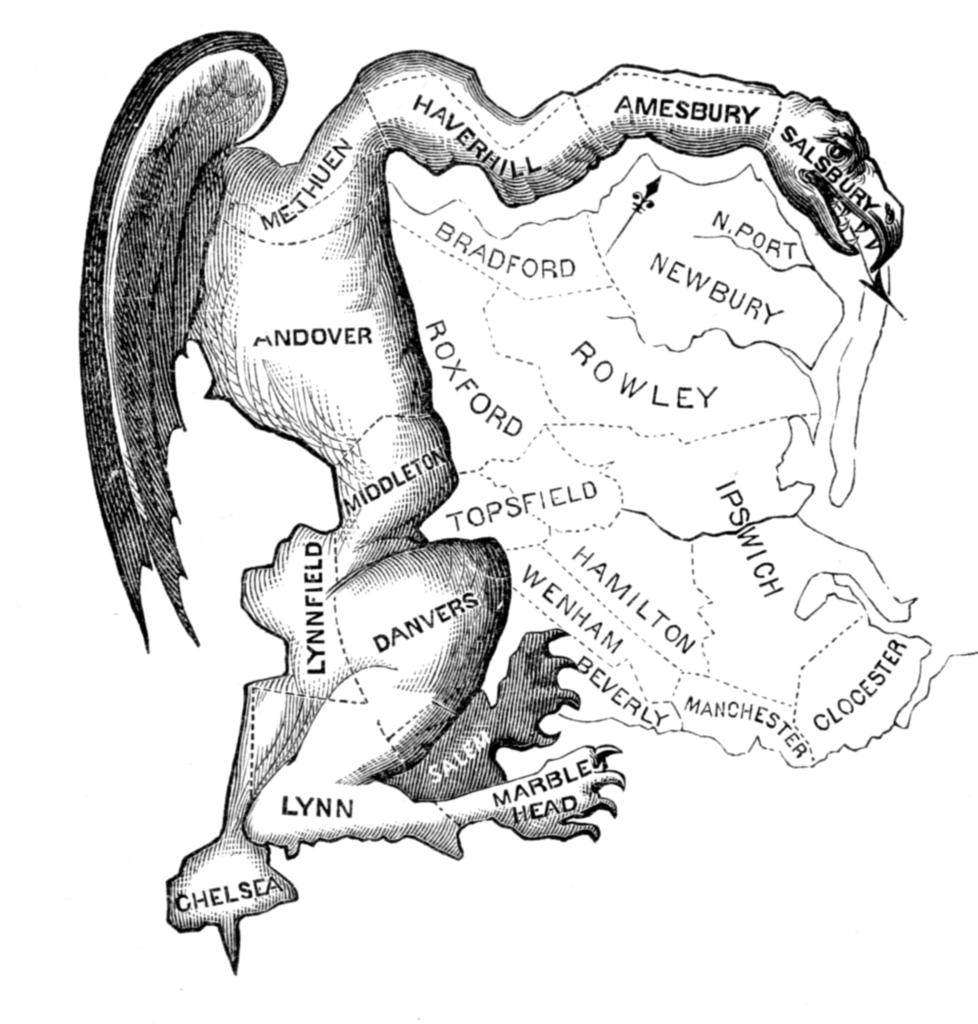
\includegraphics[width=\linewidth]{img/the-gerry-mander.png}

\column{0.5\linewidth}
In 1812, governor of Massachusetts Elbridge Gerry defined legislative districts that gave his political party an advantage.

\vspace{0.25 cm}
One of these districts was so contorted that it was called the Gerry-Mander after a mythological salamander.
\end{columns}
\end{frame}

\begin{frame}{What is gerrymandering?}
\vspace{0.35 cm}
\centering 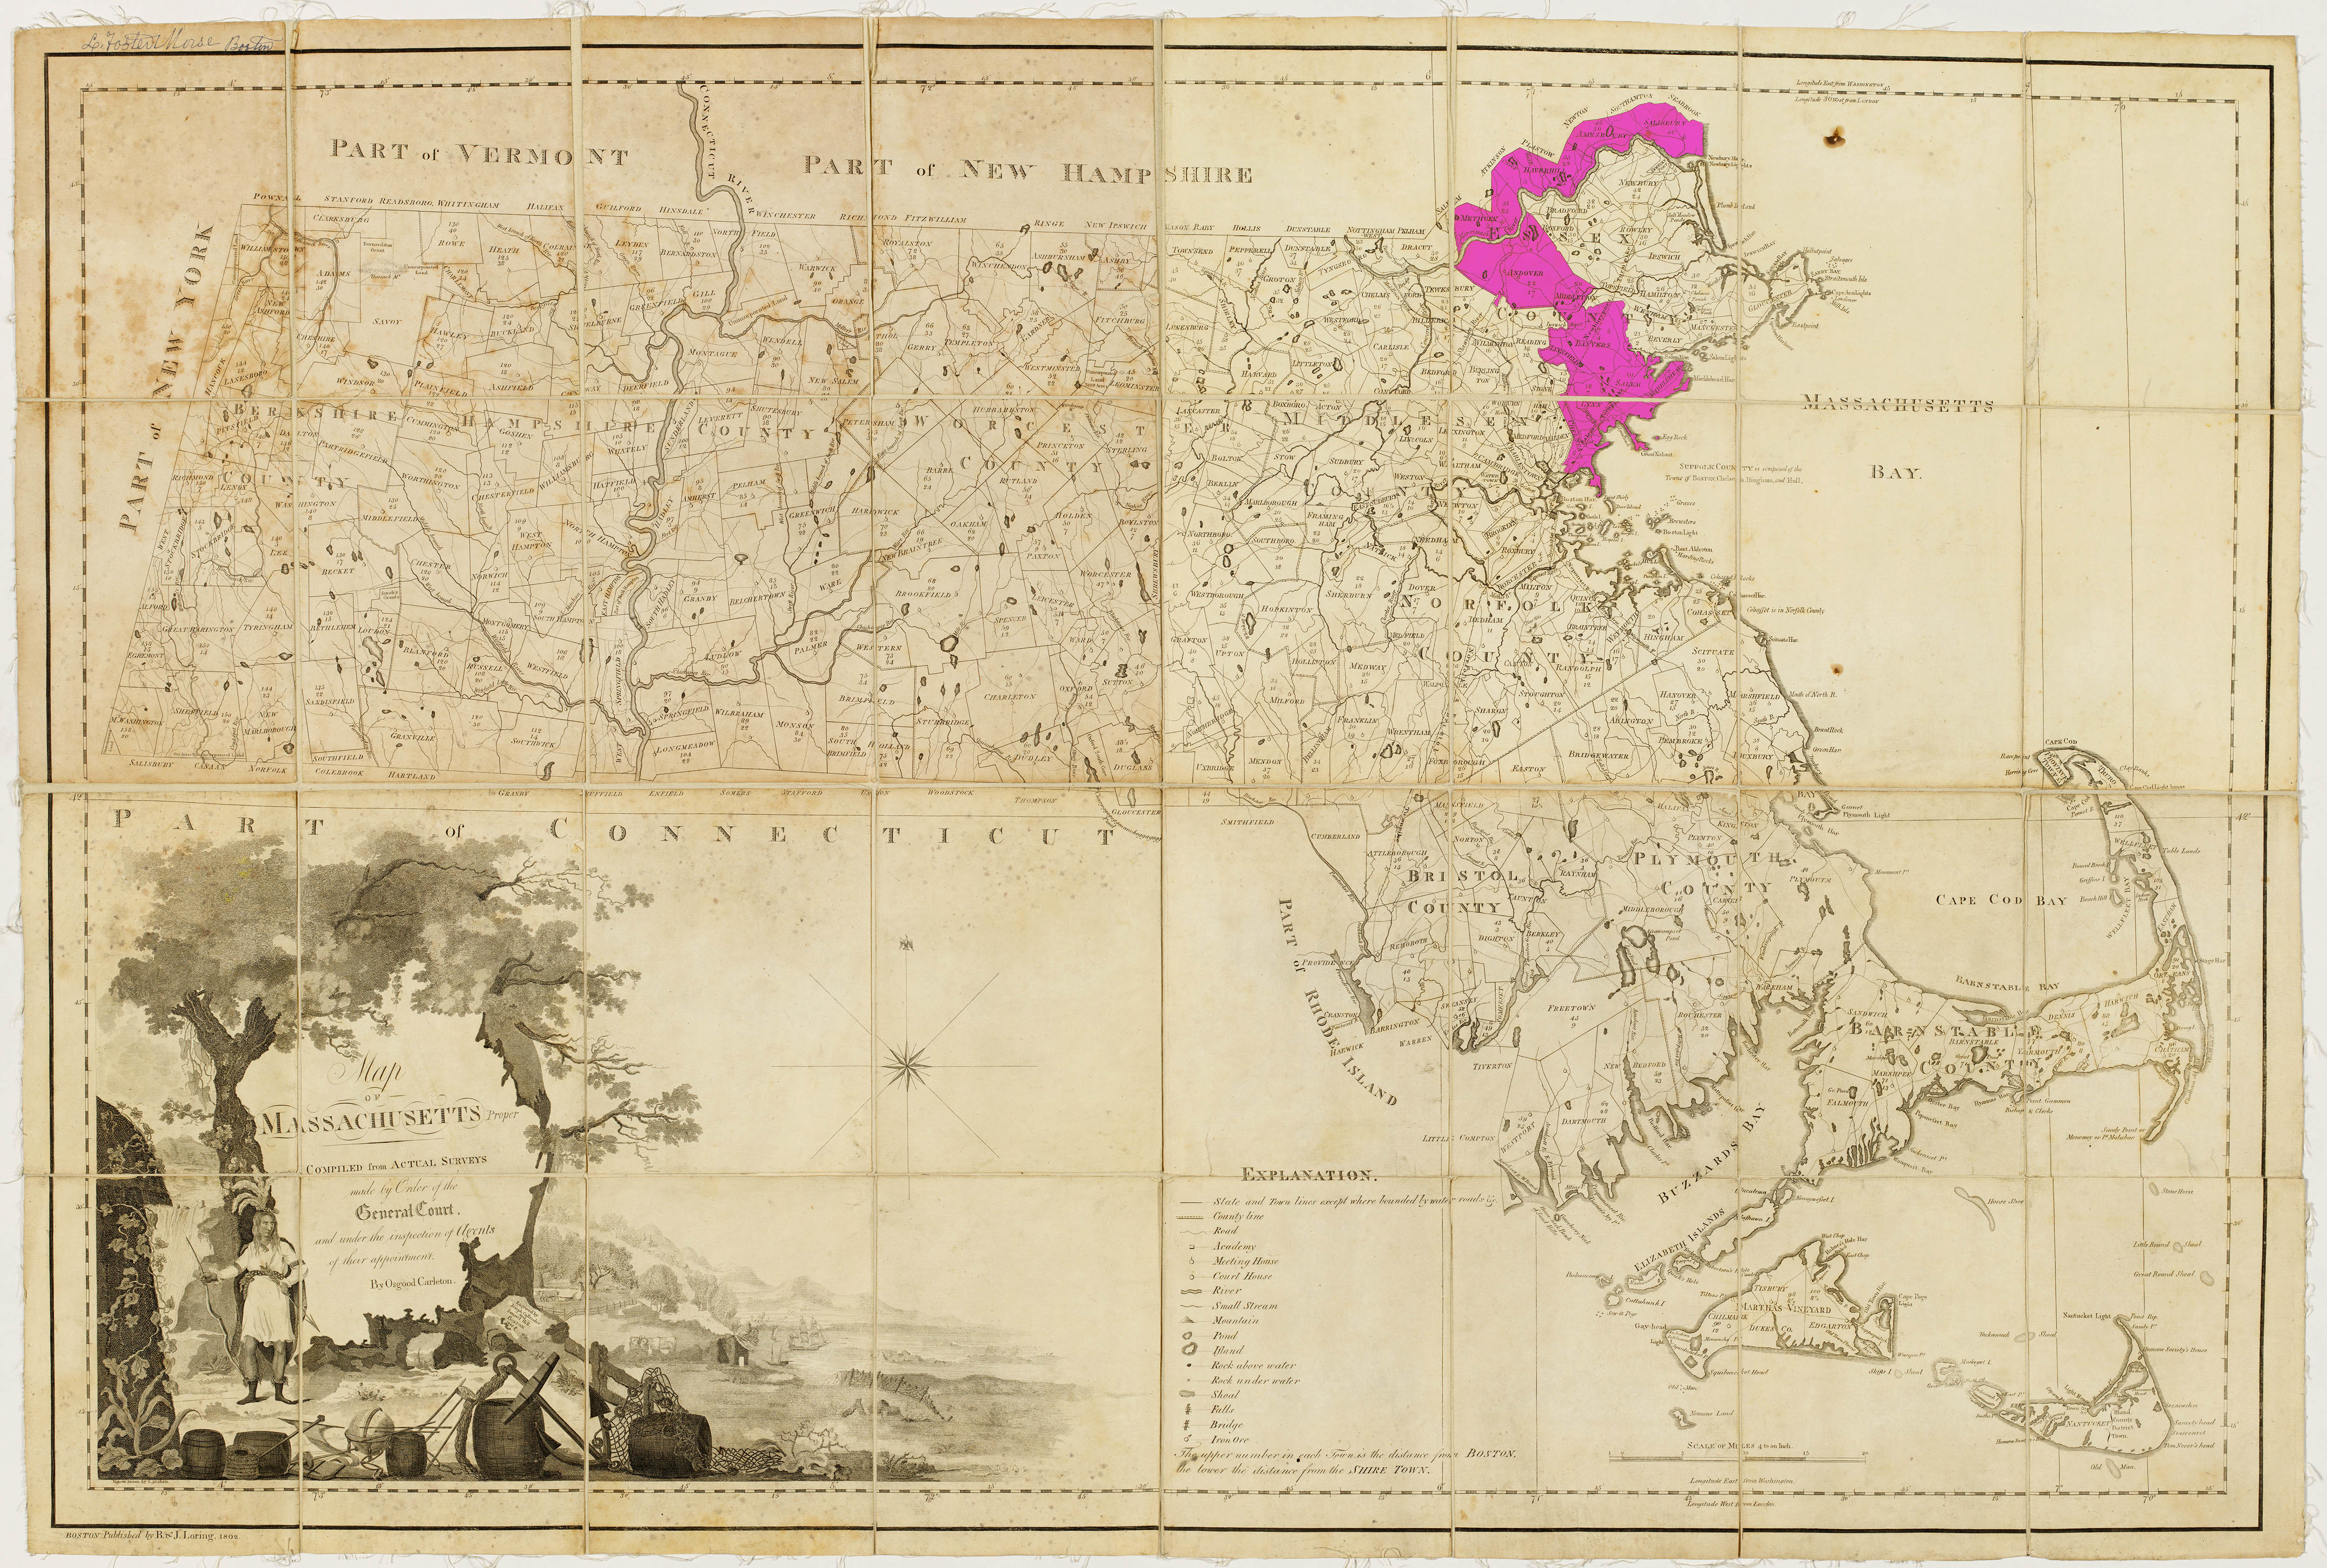
\includegraphics[width=0.8\linewidth]{img/mass-districts-1812.jpg}
\end{frame}

\begin{frame}{Washington Post's ``crimes against geography'' (2014)}
\vspace{0.35 cm}
\centering 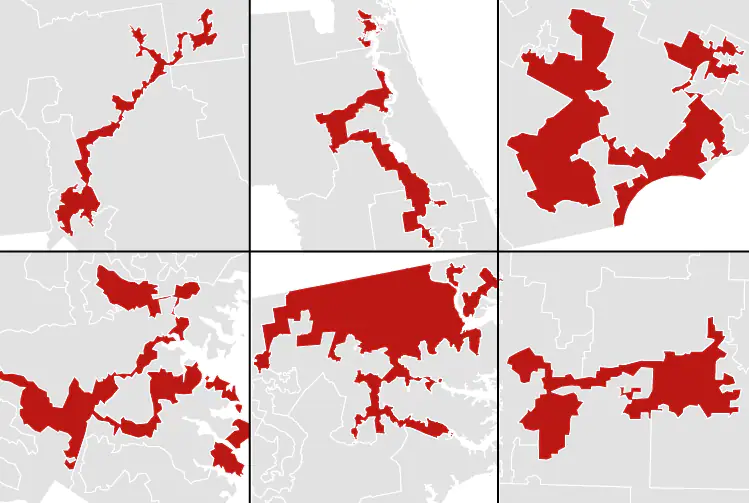
\includegraphics[width=0.8\linewidth]{img/crimes-against-geography.png}
\end{frame}

\begin{frame}{Why does shape matter?}
\vspace{0.3 cm}
\begin{columns}
\column{0.35\linewidth}
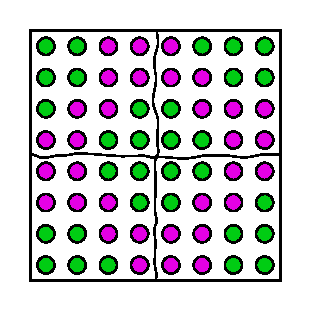
\includegraphics[width=\linewidth]{img/gerrymandering-competitive.pdf}

\centering {\bf Competitive}

Four districts are drawn without favoring any group. \phantom{Here is more text.}

\column{0.35\linewidth}
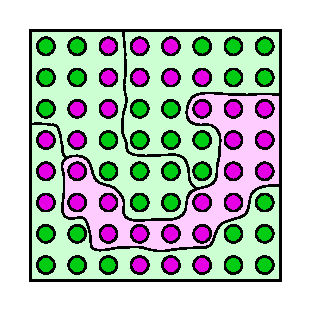
\includegraphics[width=\linewidth]{img/gerrymandering-packing.pdf}

\centering {\bf Packing}

One district absorbs all the purple so that greens can win the others.

\column{0.35\linewidth}
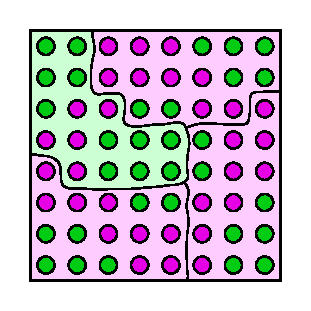
\includegraphics[width=\linewidth]{img/gerrymandering-cracking.pdf}

\centering {\bf Cracking}

Greens are split up so that they're less than a majority in most of the districts.

\end{columns}
\end{frame}




%% \begin{frame}{asdf}
%% \vspace{0.5 cm}
%% \begin{columns}
%% \column{1.1\linewidth}
%% \only<1>{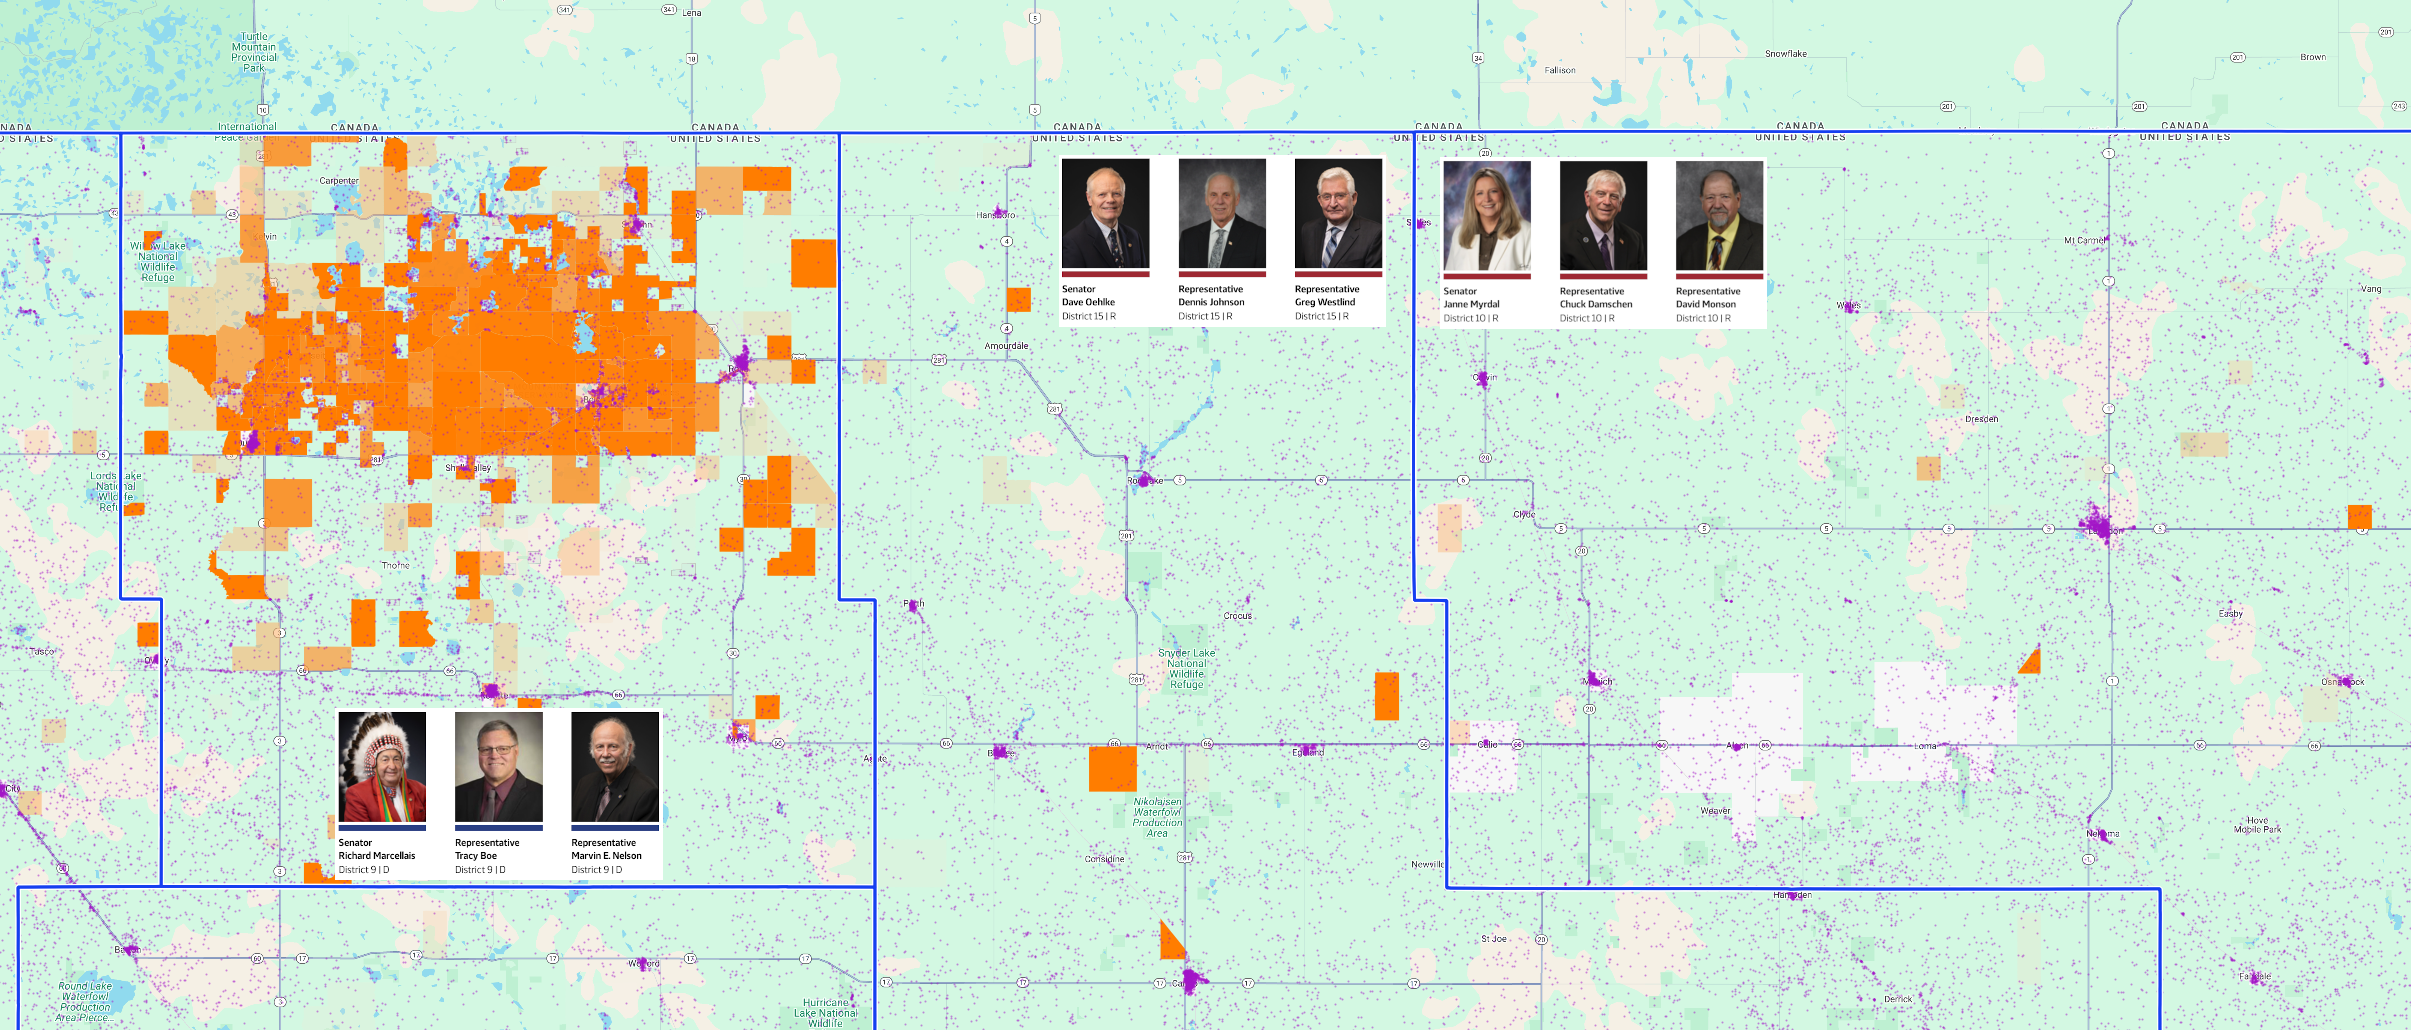
\includegraphics[width=\linewidth]{img/district-before-2022.png}}\only<2>{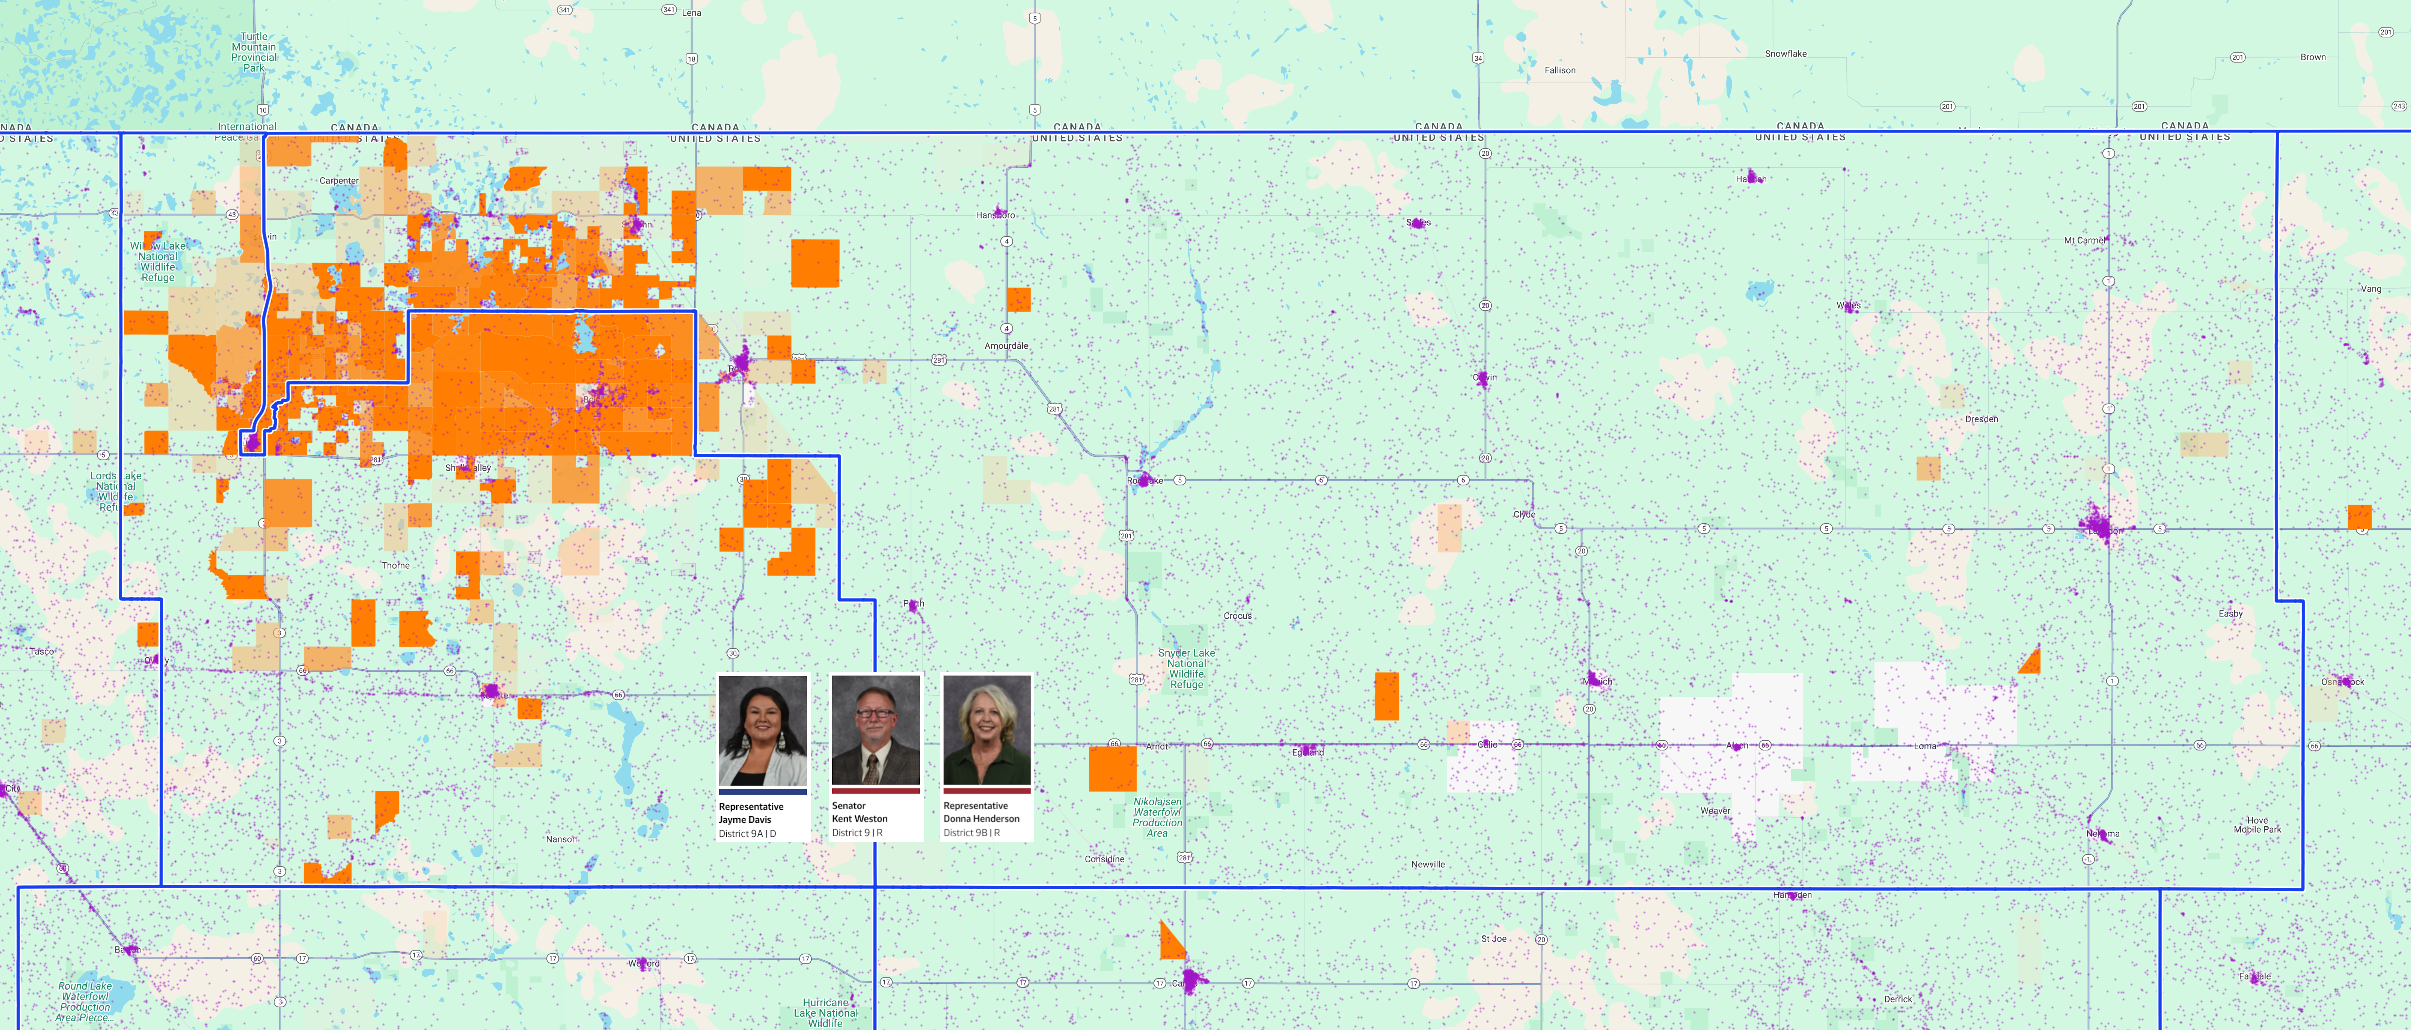
\includegraphics[width=\linewidth]{img/district-in-2022.png}}\only<3>{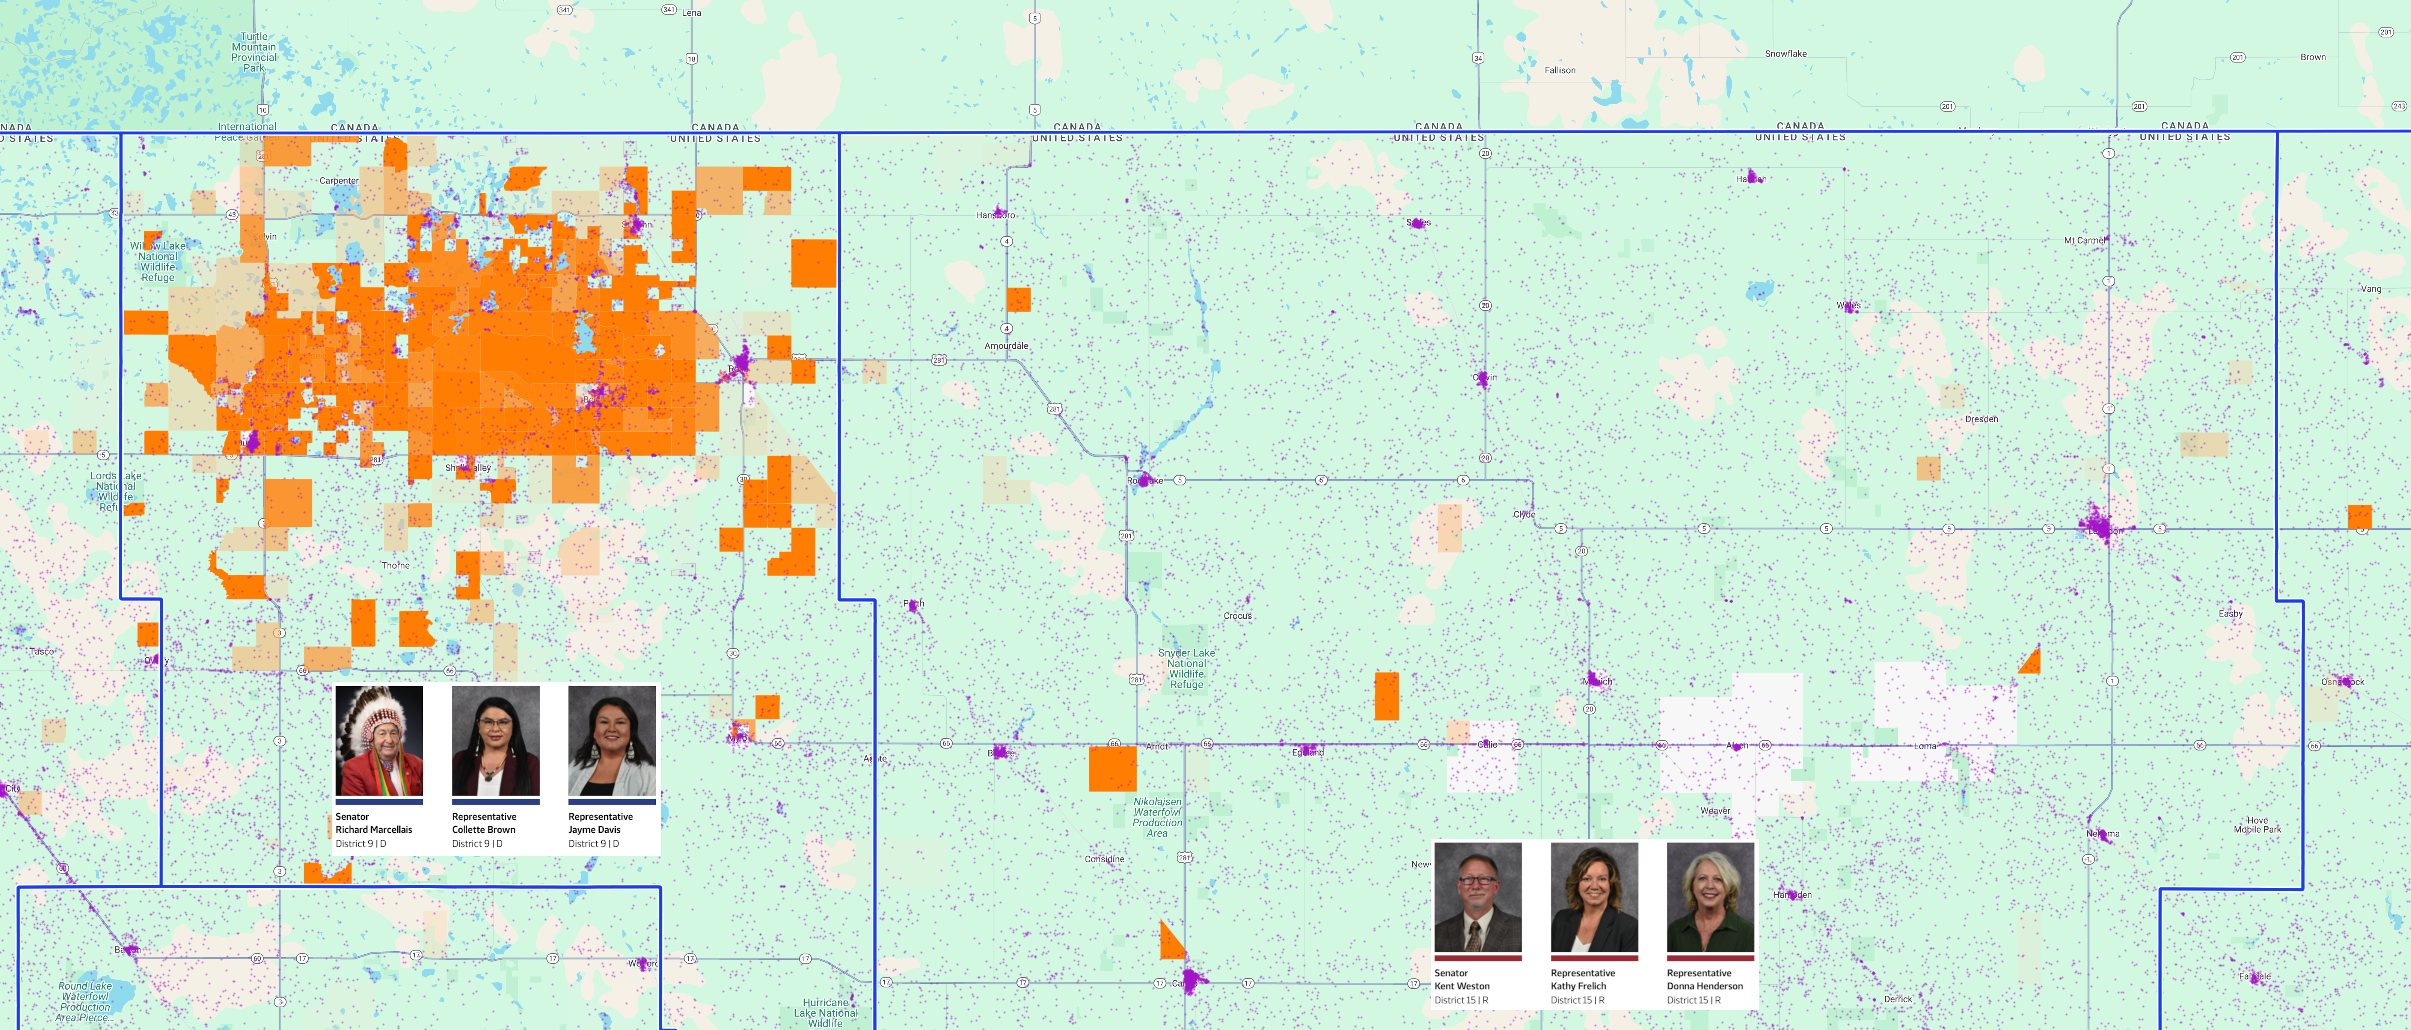
\includegraphics[width=\linewidth]{img/district-after-2022.png}}
%% \end{columns}
%% \end{frame}

\end{document}

%% https://docs.google.com/document/d/1NxDWAzdBjhC_r2hpG7xwIL2BpDFCTNYMODW7gu5YJtY/edit?tab=t.0
%% https://narf.org/cases/north-dakota-redistricting-map/
%% https://ndnativevote.org/wp-content/uploads/Redistricting-Guide.pdf

%% 0	White	nd-2024-state-senate	0.948228
%% 1	White	nd-2020-state-senate-most_competitive	0.804343
%% 2	White	nd-2020-state-senate-least_splitting	0.844429
%% 3	White	nd-2020-state-senate-most_proportional	0.856983
%% 4	White	nd-2020-state-senate-most_compact	0.857474

%% 20	Native	nd-2024-state-senate	0.610402
%% 21	Native	nd-2020-state-senate-most_competitive	2.421122
%% 22	Native	nd-2020-state-senate-least_splitting	1.978296
%% 23	Native	nd-2020-state-senate-most_proportional	1.556502
%% 24	Native	nd-2020-state-senate-most_compact	2.268171
